\section{Rotational Cooling}
\label{RC_chapter}

As has been explained in the introduction (section \ref{introduction:overview}
on page \pageref{introduction:overview}), the molecules emerging from the beam
source exist in a number of thermally-populated quantum states. We can improve
the experimental signal by concentrating as many of them as possible in a single
state. In our implementation of rotational cooling, we aim to move molecules
that have $J$ quantum numbers up to 3 down into the $J=0$ state.

This is accomplished using microwave couplings $J=1\leftrightarrow2$ and
$2\leftrightarrow3$. Then, a \UV\ laser beam centered on the $P2$ $F1$ line
(terminology defined on page \pageref{P2F1}) lifts the population from $J=2$
into the excited state $J'=1$, from where it decays down to either $J=0$ or
$J=2$. Since the $J=2$ molecules eventually get excited by the laser again, we
expect the population to accumulate in $J=0$.

\subsection{Required microwave power}

In this section, we work out an estimate of the microwave power needed to drive
rotational cooling transitions.

\subsubsection{Matrix elements}

In a simplified model of a diatomic polar molecule
\cite[sect~7.6]{budker2004atomic}, consisting of a rigid rotor, the eigenstates
are states with definite values of the angular momentum $J$ and its
$z$-projection, $m$. In the center of mass frame of the rotor, the wavefunction
is the spherical harmonic $Y_J^m(\theta,\phi)$.

The molecule-fixed dipole moment of TlF, i.e., the dipole moment along the
symmetry axis of the molecule, is $4.2\;\text{Debye}=1.7\;ea_0$
\cite[Table~1]{wilkening1984search}. Immediately making the rotating-wave
approximation, the Rabi frequency due to the applied microwave electric field
$E_0$ interacting with the dipole is (cf.  \cite[eqn~7.81]{budker2004atomic})
%
\[
    \Omega(J',m',J,m)=\frac{dE_0}{2\hbar}
    \int\limits_0^{2\pi}\d\phi
    \int\limits_0^{\pi}\d\theta\;
    Y_{J'}^{*m'}(\theta,\phi)
    \cdot\cos\theta\cdot
    Y_J^m(\theta,\phi)
    \cdot\sin\theta.
\]
%
Note that this is for $z$-polarized microwaves, and we assume $\hbar=1$. The
integral will in general be either zero or some order-unity constant. For
example, for the $J=3\rightarrow2$ transitions the integrals are
%
\[
    \frac{\Omega(2,m',3,m)}{dE_0/2\hbar}
    \approx
    \begin{pmatrix}
        0 & 0.378 & 0     & 0     & 0     & 0\\
        0 & 0.478 & 0     & 0     & 0     & 0\\
        0 & 0     & 0.507 & 0     & 0     & 0\\
        0 & 0     & 0     & 0.478 & 0     & 0\\
        0 & 0     & 0     & 0     & 0.378 & 0\\
    \end{pmatrix}_{m'm}
\]
%
We see that only the $\Delta m=0$ elements are nonzero. Finding all such
elements for $J\leftrightarrow J+1$ for $J=0,1,2,3$, we get:
\[
    \frac{\Omega(J+1,m,J,m)}{dE_0/2\hbar}
    \approx
    \begin{pmatrix}
        0     & 0     & 0     & 0.578 & 0     & 0     & 0    \\
        0     & 0     & 0.447 & 0.516 & 0.447 & 0     & 0    \\
        0     & 0.377 & 0.478 & 0.507 & 0.478 & 0.377 & 0    \\
        0.333 & 0.436 & 0.487 & 0.503 & 0.487 & 0.436 & 0.333\\
    \end{pmatrix}_{Jm}
\]
%
Thus, the Rabi frequency is approximately
%
\[
    \Omega\approx0.4\frac{dE_0}{2\hbar}.
\]

\subsubsection{Fly-through time}

Assuming (as an order of magnitude estimate) the rotational cooling region is
about 10~cm long, the flythrough time is
%
\[
    t_0\approx\frac{0.02\;\text{m}}{200\;\text{m/s}}=0.1\;\text{ms}.
\]

\subsubsection{Microwave power}

Rearranging the required condition $\Omega\gg1/t_0$, the microwave electric
field must be much greater than
%
\[
    E_0=
    \left(\frac{2\pi}{t_0}\right)
    /
    \left(\frac{0.4\;d}{2\hbar}\right)
    =2.3\;\text{V/m}.
\]
%
This corresponds to a minimum intensity
%
\[
    I_\text{min}=\frac{c\epsilon_0}{2}E_0^2\approx7.0\;\text{mW/m}^2.
\]
%
Given a waist size $w_0\approx5~\text{cm}$, the microwave power required will
have to be much greater than $P_\text{min}=\pi
w_0^2I_\text{min}=0.05~\text{mW}$.

\subsection{AR windows}

The windows of the vacuum chamber were designed to reflect as little of the
microwaves as possible while still being strong enough to withstand the
atmospheric pressure.

\subsubsection{Pressure window thickness}

The thickness of a circular window of radius $R$ required to withstand a certain
pressure $p$ is given by \cite[eqn~4.190]{moore2009building}
%
\[
    t=R\sqrt{\frac{Kp\;\text{Sf}}{Y}},
\]
%
where Sf is the safety factor (4 is adequate unless the deformation of the
window would lead to unacceptable waveform distortion). The modulus of rupture
$Y$ is about 7,000~psi for fused silica \cite{corningFS}, 65,000~psi for
sapphire \cite{sapphireWeb}. $K$ is a constant whose value can be taken as 0.75
for a clamped edge and 1.125 for a free edge.  Thus, for example, to withstand
atmospheric pressure (14.7~psi), a clamped fused silica window of radius 5~cm
would have to have a thickness of at least 8~mm.

\subsubsection{Dielectric loss}

The fraction of power transmitted through a window is subject to dielectric loss
in the window. As it propagates a distance $z$ into the window, the power
(normalized to input power) decays as
%
\[
    P(\delta,\lambda,z)=\exp\left(-\delta\frac{2\pi}{\lambda}z\right),
\]
%
where the wavelength in the dielectric material is $\lambda=c/(nf)$, and
$\delta$ is the loss angle, commonly quoted as the loss tangent $\tan\delta$.
For fused silica, $\tan\delta\approx0.0003$.  The dielectric loss, which causes
the frequency dependence, is a negligible effect. E.g., going through a 10~mm
thick window, it would be about 0.2\%\ to 0.6\%\ at our frequencies.  Since this
is merely radiation lost as heat (as opposed to microwaves), a 1\% power loss is
tolerable and can be ignored in what follows.

\subsubsection{Coherence length}

For light passing through a glass window, we normally cannot observe thin film
interference, since the coherence length or sunlight ($\approx0.6\;\mu$m) is
much smaller than the window thickness (a few millimeters).

However, coherence length being inversely proportional to the bandwidth, it is
much greater in the microwave range. For example, a source with a 1~MHz frequency
uncertainty would have a vacuum coherence length of
$L=c/1\;\text{MHz}=300~\text{m}$.

\subsubsection{Reflectance and interference at normal incidence}

In this section, we express the reflectivity of a window in terms of the
characteristic admittance $Y$, which is simply the reciprocal of
characteristic impedance: $Y=1/Z$. The two quantities relate the magnitudes
$|\vec E|$ and $|\vec H|$ of electric and magnetic fields, respectively, of
electromagnetic radiation traveling through some medium. For example, the
admittance of free space is $y_0\approx2.65\cdot10^{-3}$~S
\cite[eqn~2.25]{macleod2017thin}.

The phase change for planar wavefronts at normal incidence across a window of
thickness $d$ and refractive index $n$ will be $\delta=2\pi nd/\lambda_0$, where
$\lambda_0$ is the vacuum wavelength. The admittance of the window is given by
\cite[eqn~2.93]{macleod2017thin}
%
\begin{equation}
    \label{win_admittance}
    Y=\frac{y_0\cos\delta+iy_1\sin\delta}{\cos\delta+i(y_0/y_1)\sin\delta},
\end{equation}
%
where $y_0$ is the admittance of free space, while for an ideal dielectric
window of permittivity $\epsilon_1$ and permeability $\mu_1$, its admittance will be $y_1=\sqrt{\epsilon_1/\mu_1}$. Since for
dielectrics, $\mu\approx\mu_0$, we can assume
$y_1\approx\sqrt{\epsilon_1}y_0$. For fused silica,
$y_1\approx\sqrt{3.8}y_0$.

The corresponding power reflectivity is \cite[eqn~2.91]{macleod2017thin}
%
\begin{equation}
    \label{win_refl}
    R=\Big|\frac{y_0-Y}{y_0+Y}\Big|^2
\end{equation}
%
A 5~mm thick fused silica window would thus have the reflectivity shown in
Fig.~\ref{AR_win_p1}. We see that unless the window thickness is matched to the
frequencies of the radiation we use, the window can reflect up to 35\%\ of
incident power. However, when the frequency is matched, ideally no power is
reflected at all. Even if we change the frequency by 1.6~GHz from each minimum,
the reflectivity will stay below 5\%.

\begin{figure}
    \centering
    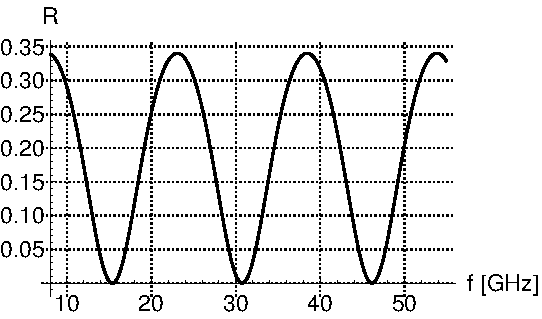
\includegraphics[width=.7\textwidth]{figs/mathematica/AR_win_p1.pdf}
    \caption[Window reflectivity vs microwave frequency.]{Reflectivity of a 5~mm
    thick fused silica ($\epsilon_\text{r}=3.8$) window exposed to microwave
    radiation at normal incidence.}
    \label{AR_win_p1}
\end{figure}

\subsubsection{Half-wave windows}

Due to the periodicity of the reflection coefficient, we only need a single
window thicknesses to cover our three microwave frequencies (13.4 GHz, 26.8 GHz,
40.1 GHz), namely the half-wave thickness 5.75~mm (or a multiple of this
thickness). Indeed, it is a well known fact that a stack containing an integer
number of half-wave layers has no effect on reflectance or transmittance of
assemblies, at wavelengths at which they are truly half-wave. Thus ``half-wave
layers are sometimes referred to as absentee layers''
\cite[sect~2.9]{macleod2017thin}.

As explained above, the window has to be at least 8~mm thick to withstand the
atmospheric and other forces. That is why an integer multiple of the thickness
has to be chosen, such as $2\times5.747~\text{mm}=11.494~\text{mm}$.
Unfortunately, the windows used in \CENTREX\ to date (Jun 2023) were ordered as
$(11.762\pm0.12)$~mm thick owing to a confusion in calculating the wavelength
in vacuum vs in the material ($\sqrt{3.8}\approx1.95\approx2$). Besides, it is
not clear how close to 3.8 the relative permittivity actually is; it would be
interesting to measure the reflectivity of several windows in the thickness
range of, say, 5\%\ around the predicted optimal thickness of 11.50~mm.

\subsubsection{Residual reflectivity}

The lower bound for reflectivity is realistically set by how precisely the
window thickness can be controlled. It can be kept below 1\%\ if the window
thickness can be within about $\pm2~\text{mil}=0.05~\text{mm}$, as seen in
Fig.~\ref{AR_win_p2}.

\begin{figure}
    \centering
    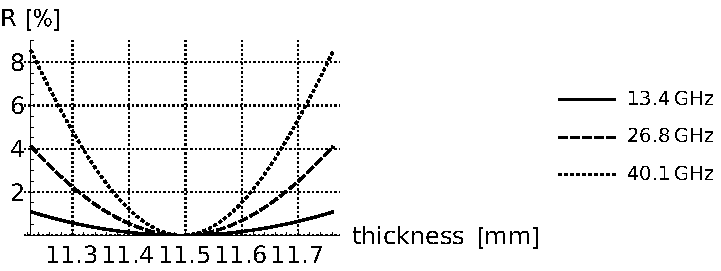
\includegraphics[width=.7\textwidth]{figs/mathematica/AR_win_p2.pdf}
    \caption[Residual microwave reflectivity vs window thickness.]{Residual
    microwave reflectivity when the window ($t=11.494$~mm) is not of the optimal
    thickness. The actual window thickness, 11.762~mm, corresponds to the
    rightmost point of the horizontal axis. This plot assumes the refractive
    index of $\sqrt{3.8}$.}
    \label{AR_win_p2}
\end{figure}

Of course, this assumes a particular value of the refractive index. For fused
silica, the refractive index is given by one reference as $1.812\pm0.003$ at
94.3~GHz, and 1.949 at 105.3~GHz \cite[Table~5.1]{goldsmith1998quasioptical}.
Another reference \cite{popovic2019materials} gives the relative permittivity of
$3.80\pm0.02$ from 5 to 110~GHz, which corresponds to a refractive index of
$1.95\pm0.005$. Whatever the exact material used, its refractive index needs to
be known precisely in order to determine the exact optical thickness of the
window (Fig.~\ref{AR_win_p3}).

\begin{figure}
    \centering
    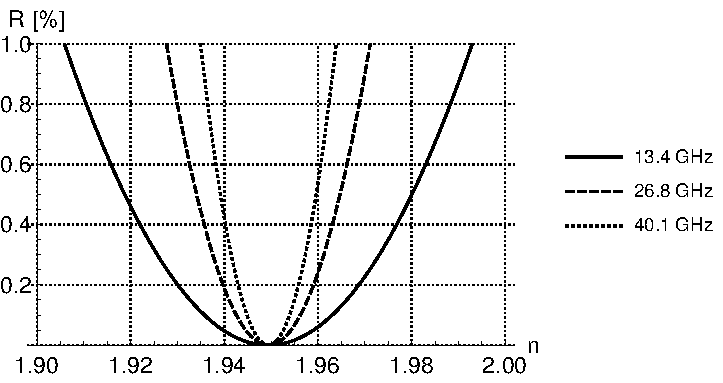
\includegraphics[width=.7\textwidth]{figs/mathematica/AR_win_p3.pdf}
    \caption[Residual reflectivity vs refractive index.]{Residual microwave
    reflectivity versus refractive index variations, for window thickness
    $t=11.494$~mm.}
    \label{AR_win_p3}
\end{figure}

The frequency bandwidth to keep R below 1\%\ is about 1.2~GHz as seen in
Fig.~\ref{AR_win_p4}.

\begin{figure}
    \centering
    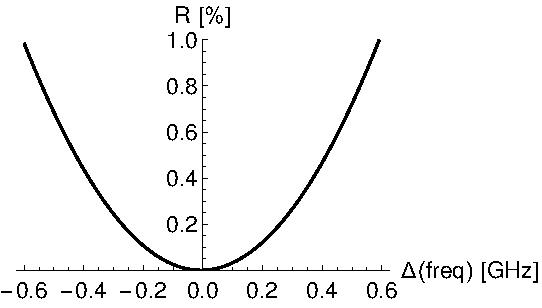
\includegraphics[width=.7\textwidth]{figs/mathematica/AR_win_p4.pdf}
    \caption[Residual reflectivity vs microwave frequency.]{Residual
    reflectivity versus microwave frequency variations, for window thickness
    $t=11.494$~mm.}
    \label{AR_win_p4}
\end{figure}

\subsubsection{Oblique incidence}

For waves incident on the windows at an oblique angle $\theta$, equations
\ref{win_admittance} and \ref{win_refl} still hold, except that now the phase
change for waves going cross the window is modified to $\delta=2\pi
nd\cos\theta/\lambda_0$. The reflectivity as a function of angle is shown in
Fig.~\ref{AR_win_p5}.

\begin{figure}
    \centering
    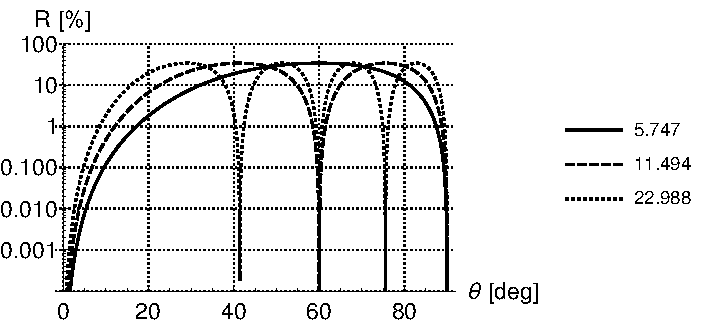
\includegraphics[width=.7\textwidth]{figs/mathematica/AR_win_p5.pdf}
    \caption[Residual reflectivity versus angle of incidence.]{Residual
    reflectivity versus angle of incidence. The legend shows the three window
    thicknesses listed in the plot legend (in units of mm). Index of
    refraction is assumed to be $\sqrt{3.8}$.}
    \label{AR_win_p5}
\end{figure}

While the microwaves are launched at normal incidence to the window given the
relative orientation of the horns and windows, the oblique incidence effect can
be significant when the waves get reflected from metallic objects, such as the
vacuum chamber, or if the wavefronts themselves are curved. We will now estimate
the effect due to curvature, while the chamber reflections are considered in the
next section.

For a Gaussian beam of waist $w_0$ at a distance $z$ away from the waist, we
have the beam radius of curvature $R$ and width $w$
\cite[eqn~2.21]{goldsmith1998quasioptical}:
%
\begin{align}
    \label{radius_width}
    R=z+\frac{1}{z}\left(\frac{\pi w_0^2}{\lambda}\right)^2
    ;\quad
    w=w_0\sqrt{1+\left(\frac{cz}{\pi w_0^2f}\right)^2},
\end{align}
%
where $\lambda$ is the wavelength, $f$ is the frequency, and $c$ is the speed of
light. (In this experiment, typical values are $w_0=1$~in, $f=14$~GHz.)

The beam intensity at a transverse position $r$ is
\cite[eqn~2.25]{goldsmith1998quasioptical}:
%
\begin{align}
    \label{Gaussian_intensity}
    I&=I_0\left(\frac{w_0}{w}\right)^2\exp\left(-\frac{2r^2}{w^2}\right).
\end{align}
%
The angle of incidence $\theta$ and the transverse position $r$ are related via
the radius of curvature $R$ as $r=R\cos(\pi/2-\theta)$. Thus we can plot the
beam intensity as a function of the angle of incidence on the same plot as
reflectivity vs angle (Fig~\ref{AR_win_p6}). The beam intensity decreases with
increasing distance from the beam axis (and hence, with angle of incidence). At
the same time, the reflectivity increases. 

\begin{figure}
    \centering
    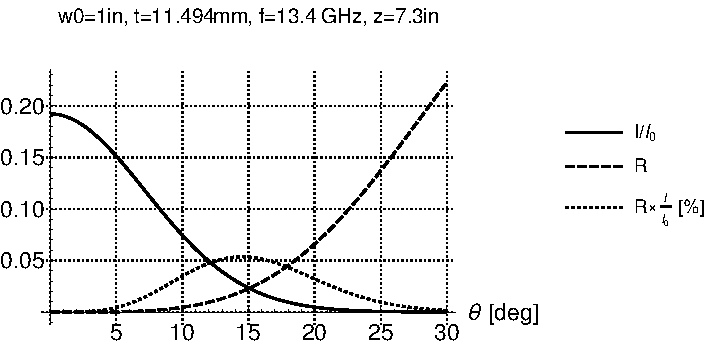
\includegraphics[width=.7\textwidth]{figs/mathematica/AR_win_p6.pdf}
    \caption[Residual reflectivity due to wavefront curvature.]{Residual
    reflectivity due to wavefront curvature. Note that all quantities are
    dimensionless and therefore plotted on the same vertical axis. The window
    index of refraction is assumed to be $\sqrt{3.8}$.}
    \label{AR_win_p6}
\end{figure}

The outer parts of the beam will be reflected much more than the beam centre.
However, the beam intensity near the outer parts of the window is greatly
reduced since most of the beam power is near the centre. Thus, the actual power
reflected from the edges of the windows due to the beam curvature is negligible.

\subsection{Clipping}

Ideally, perfectly Gaussian beams would be used with infinite windows. In
practice, the vacuum chamber geometry requires the windows to be a finite size.
Inevitably, a fraction of the power of the beam would get clipped at the edges
of the windows. In this section, we calculate the diameters of the windows
needed to lose an acceptable amount of the beam power.

According to eqn~\ref{Gaussian_intensity}, the beam intensity decays
exponentially as $\exp(-2r^2/w^2)$ with the transverse position $r$ away from
the beam axis, given a certain beam waist $w$ (defined in
eqn~\ref{radius_width}). If we want the intensity at the edge of the windows to
be, say, 0.25\%\ of the intensity at the center of the beam, then the window
diameter $D$ needs to be
%
\[
    D>2w\sqrt{-\frac{\ln0.0025}{2}}\approx3.5\;w,
\]
%
where the beam width $w$ is given in eqn~\ref{radius_width}. The vacuum chamber
as built (Fig.~\ref{RCch}) has three pairs of identical microwave windows. The
two holes for 13.4~GHz microwaves have a diameters of 8.150" and are separated
by 14.58", while the other two pairs (for 26.8 and 40.1~GHz) both have a 5.450"
diameter and are separated by 16.13". The chamber also has a pair of 2" holes
for a laser, as well as the connection for the molecular beam, perpendicular to
all the laser and microwave beams. With these dimensions, the clipping of the
the 1"-waist microwave beams is kept below 0.2\%.

The vacuum connection is an ISO200 F-style flange on one side, and a custom
``Input Nipple'' on the other (3/4" long nipple, 2.87" ID, flange 5.8" OD and
1/4" thick).  The custom flange was originally intended to be used as a part of
a sliding vacuum seal to allow for beamline alignment while being very compact
in size.  The sliding seal never got designed or made, and instead we use
bellows to obtain the same flexibility.

\begin{figure}
    \centering
    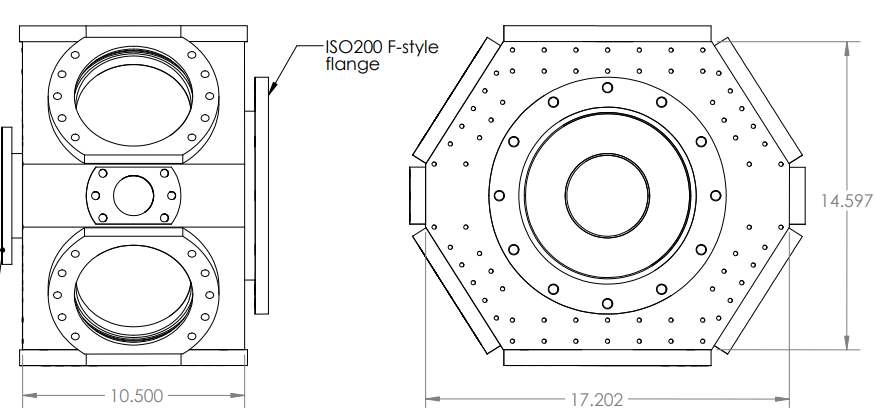
\includegraphics[width=\textwidth]{figs/todo/RCch.png}
    \caption{RC chamber}
    \label{RCch}
\end{figure}

\subsection{Beam-blocking mesh}

The microwaves in the rotational cooling region interfere with other
experimental regions further down the beamline and need to be blocked from
entering those regions without blocking the molecular beam. This can be
accomplished using a metallic mesh.

We model the mesh as two perpendicular array of parallel wires, since ``the
behavior of the two-dimensional grid can be calculated purely from that of its
constituent one-dimensional inductive grid''
\cite[p.~242]{goldsmith1998quasioptical}.

Consider infinite-length wires of radius $a$, permeability $\mu_1$, and
conductivity $\sigma=1/\rho$ (which is the reciprocal of resistivity $\rho$),
arranged in an array with spacing $d$. The reflection coefficient for radiation
of frequency $\omega=2\pi f$ and wavelength $\lambda=c/f$ at normal incidence is
\cite[eqns~24--25]{wait1955reflection}
%
\[
    R=\frac{-1}{1+2Z_\text{g}/Z_0},
    \quad
    Z_\text{g}=iZ_0\frac{d}{\lambda}
    \left[\ln\frac{d}{2\pi a}+F(d/\lambda,0)\right]
    +Z_\text{i}d,
\]
%
where $Z_0\approx376.7~\Omega$ is the impedance of free space and
\cite[eqn~17 and 22]{wait1955reflection},
%
\begin{align*}
    Z_\text{i}\approx
    \sqrt{\frac{\mu_1\omega}{2\sigma}}
    \left(\frac{1+i}{2\pi a}\right)
    ,\quad
    F\left(\frac{d}{\lambda},0\right)=
    \sum_{m=1}^\infty\Big(\frac1{\sqrt{m^2-(d/\lambda)^2}} - \frac1m\Big)
    .
\end{align*}
%
The mesh used in the experiment is made of copper (Precision Electroforming
MC12, 0.53~mm wire spacing, 17.5~$\mu$m wire radius). The transmission
$T\approx1-|R|^2$ of 26.7~GHz microwaves through such a grid is shown in
Fig.~\ref{wires}. 

\begin{figure}
    \centering
    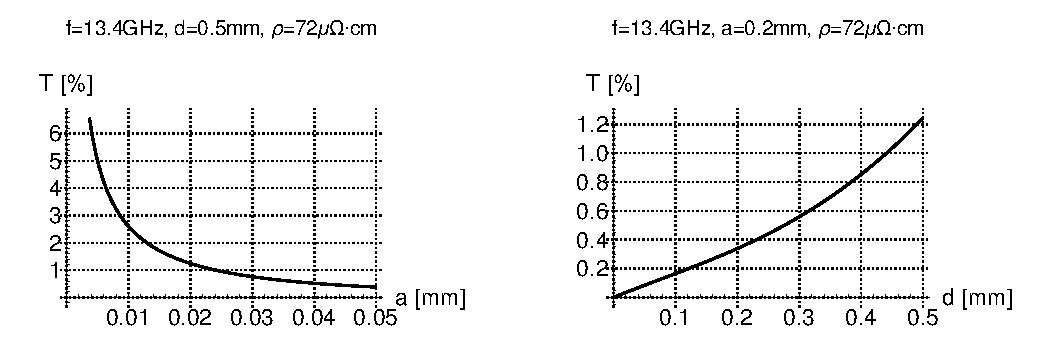
\includegraphics[width=\textwidth]{figs/mathematica/wires.pdf}
    \caption[Microwave transmission through wire mesh.]{Transmission of 13.4~GHz
    microwaves at normal incidence through a copper wire mesh. Here
    $\mu_1=\mu_0$.}
    \label{wires}
\end{figure}

The attenuation of the 26.7~GHz microwaves through this mesh was measured to be
approx.\ 13~dB \cite[sect~6.3]{timgren2023thesis}, or about 5\%\ transmission,
which is more than the $\approx2$\%\ shown in the plot in Fig.~\ref{wires}. It
is possible that some of the microwave power found its way around the mesh,
either because the mesh was not properly sealed against the chamber aperture, or
because the microwaves were transmitted ouf through the laser windows of one
chamber and again through the windows into the next one.
